\Needspace{3in}
\begin{prob}

    Suppose Dijkstra's algorithm is run on the graph shown below using node $a$ as the source.

    \begin{center}
        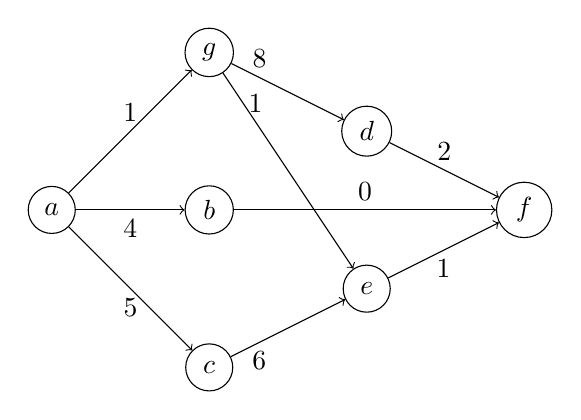
\begin{tikzpicture}
            {
                \tikzset{every node/.style = {shape=circle, draw, minimum size=17pt}}

                \node (a) at (0, 0) {$a$};
                \node (g) at (2, 2) {$g$};
                \node (b) at (2, 0) {$b$};
                \node (c) at (2, -2) {$c$};
                \node (d) at (4, 1) {$d$};
                \node (e) at (4, -1) {$e$};
                \node (f) at (6, 0) {$f$};
            }

            % draw an edge with label in the middle
            \draw (a) edge[->] node[above, midway] {1} (g);
            \draw (a) edge[->] node[below, midway] {5} (c);
            \draw (a) edge[->] node[below, midway] {4} (b);
            \draw (g) edge[->] node[above, near start] {8} (d);
            \draw (g) edge[->] node[above, near start] {1} (e);
            \draw (b) edge[->] node[above, midway] {0} (f);
            \draw (c) edge[->] node[below, near start] {6} (e);

            \draw (d) edge[->] node[above, midway] {2} (f);
            \draw (e) edge[->] node[below, midway] {1} (f);

        \end{tikzpicture}
    \end{center}

    Suppose $C$ is the set of ``correct'' nodes: that is, $C$ is the set of nodes whose estimated distances
    are known to be correct.

    What will be the fifth node added to $C$ by Dijkstra's algorithm? (The
    first node added to $C$ is the source, $a$.)

    \inlineresponsebox[.75in]{$b$}

\end{prob}
